\documentclass{article}
\usepackage[polish]{babel}
\usepackage[a4paper, margin=2cm]{geometry}
\usepackage{graphicx}
\usepackage{polski}
\usepackage[utf8]{inputenc}
\usepackage{lettrine}
\usepackage{xcolor}
\usepackage[nodayofweek]{datetime}
\renewcommand{\familydefault}{\sfdefault}

\usepackage[autocite=superscript]{biblatex}
\addbibresource{bibliography.bib}

\title{Historia boulderingu i jego pięć znaczących postaci}
\author{Marcin Młynarczyk}
\newdate{date}{11}{6}{2020}
\date{\displaydate{date}}
\definecolor{blue}{cmyk}{.6,.28,0,.04}

\usepackage{sectsty}
\chapterfont{\color{blue}}
\sectionfont{\color{blue}}
\subsectionfont{\color{blue}}

\addto\captionspolish{
  \renewcommand{\contentsname}%
    {\color{blue}Spis treści}%
}

\begin{document}

\maketitle
\tableofcontents

\bigskip

\begin{figure}[!htbp]
	\begin{center}
		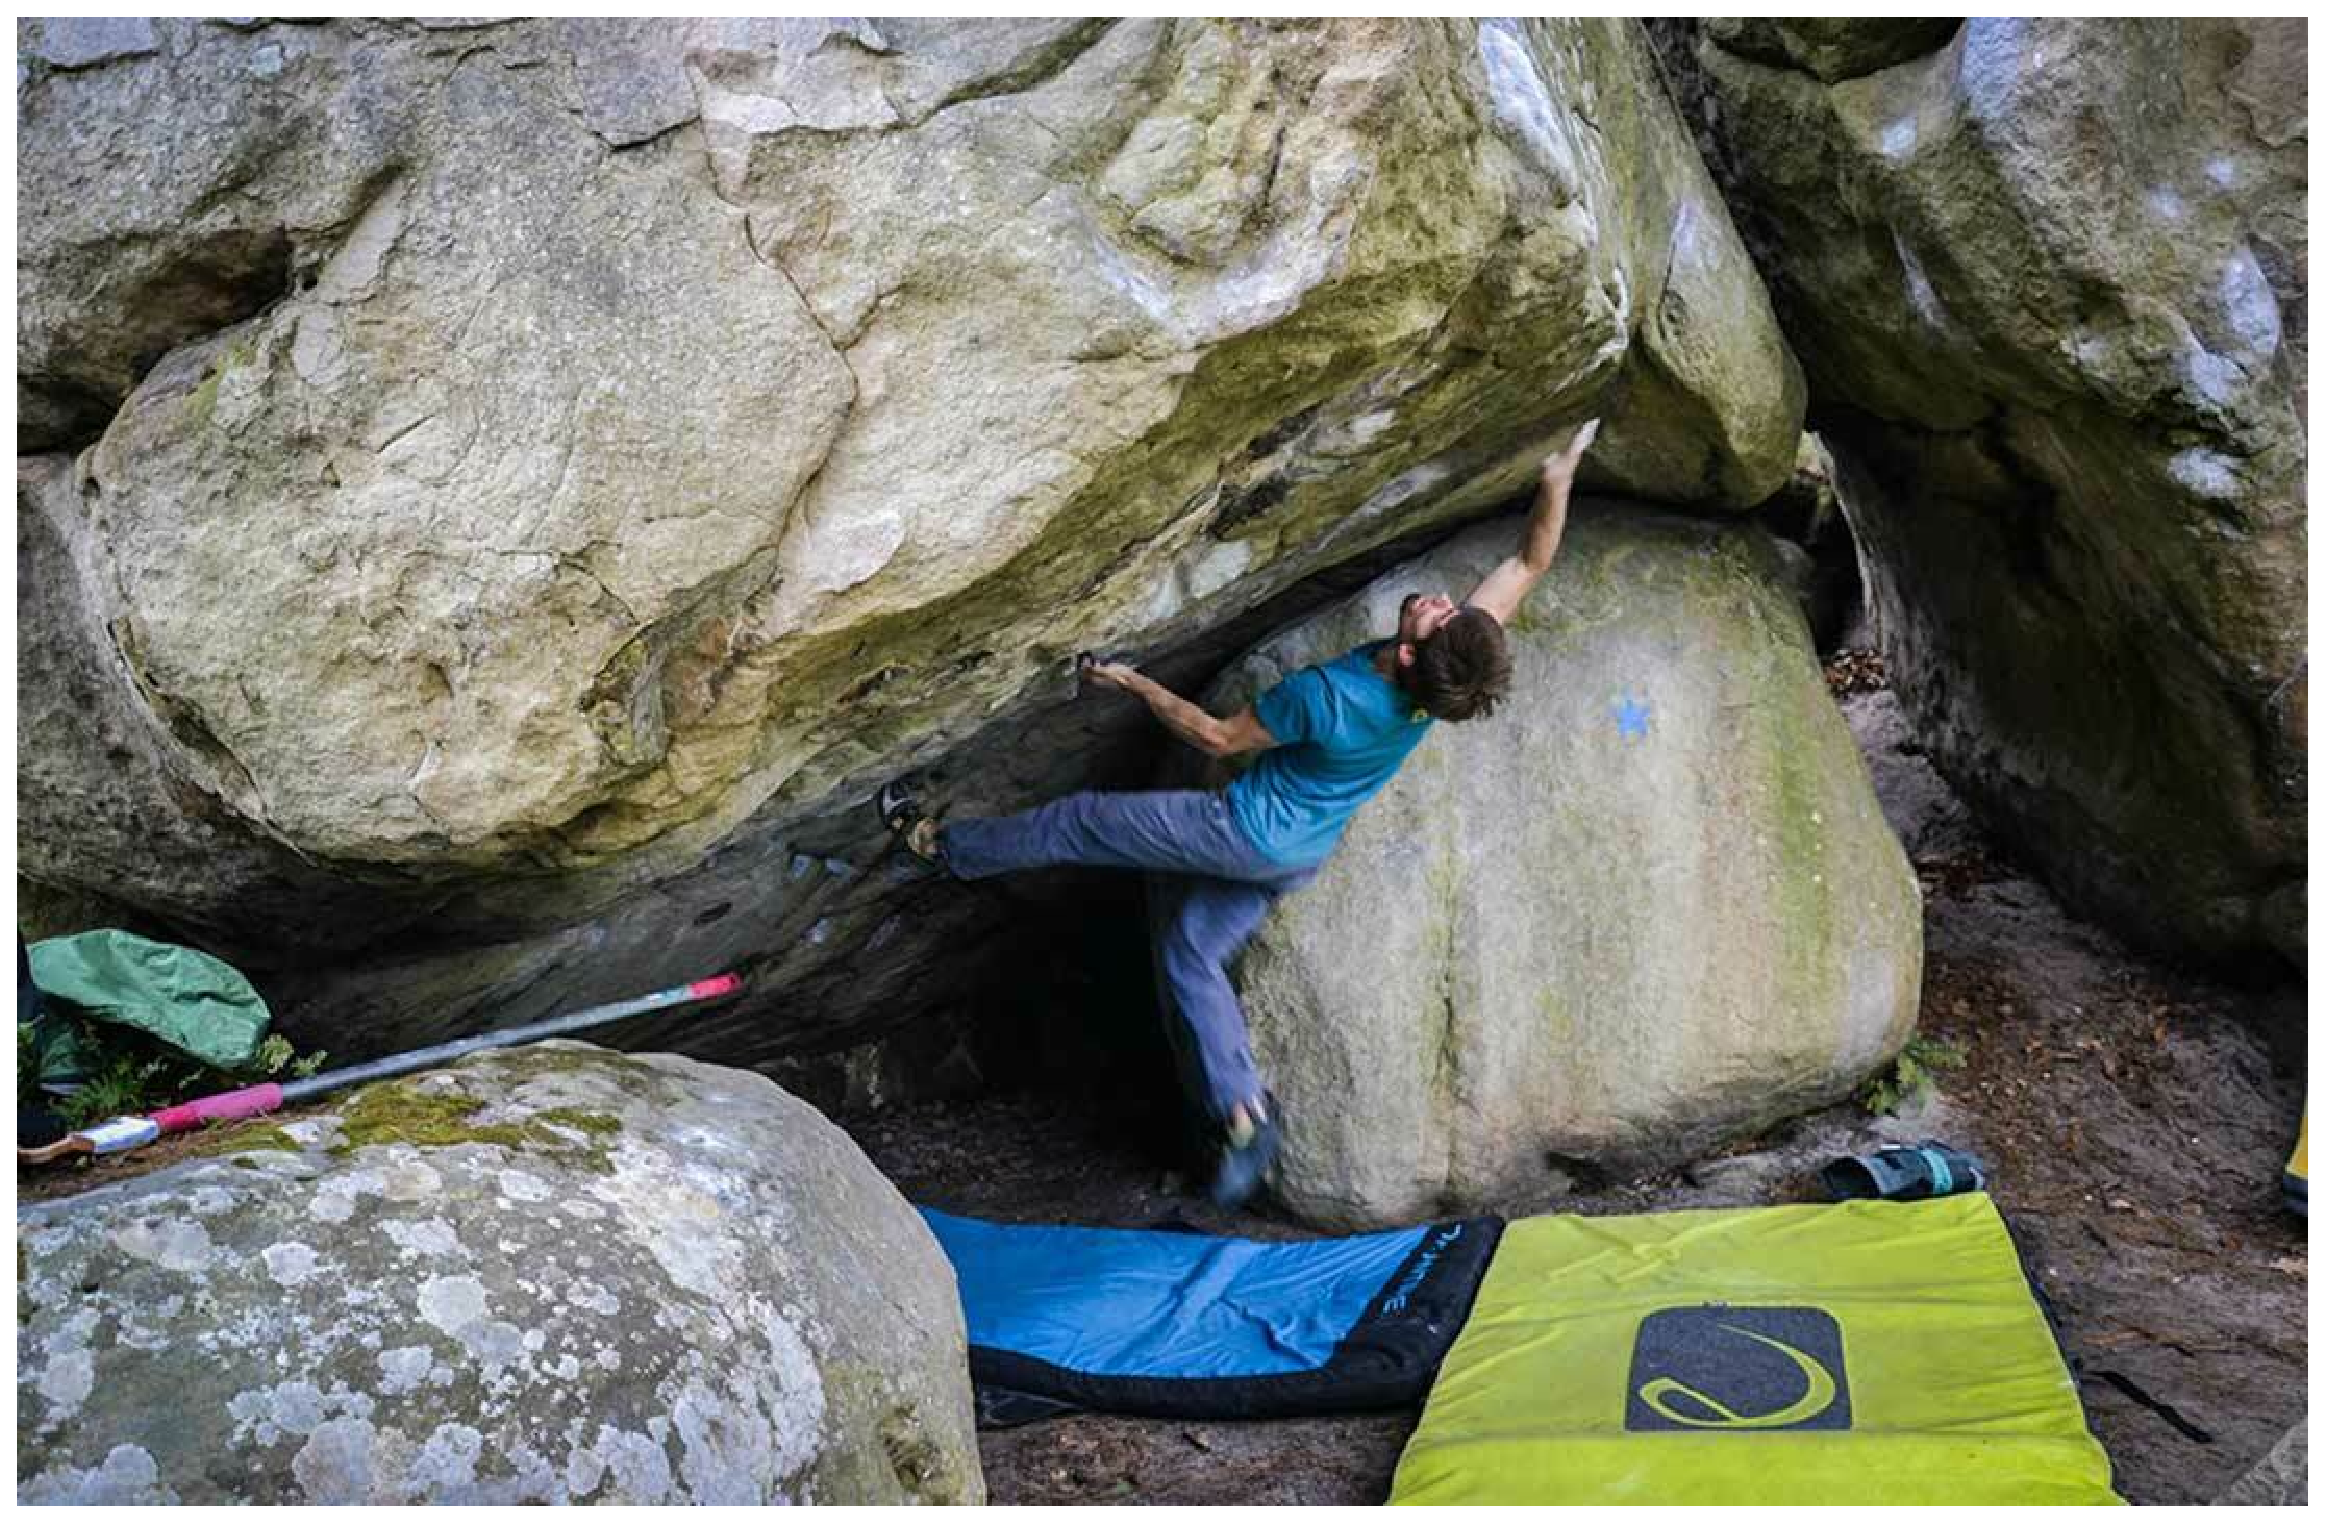
\includegraphics[width=0.7\linewidth]{images/intro.eps}
	\end{center}
	\caption{Roman Batsenko na Gourmandise Raccourci 8A+, \textit{Fontainebleau}, Francja (fot. Karolina Stawoska) \cite{8a}}
\end{figure}

\section{Wstęp}
\lettrine[lines=2]{B}{ouldering} staje się coraz popularniejszą formą aktywności fizycznej. Owy termin, w swojej angielskiej postaci, dość mocno zakorzenił się w polskim żargonie wspinaczkowym. Pojęcie \textit{bouldering} pochodzi z języka angielskiego, w którym oznacza \textit{głaz}. Zatem uprawianie boulderingu to w dosłownym tłumaczeniu "głazowanie", czyli wspinanie się na głazy. W języku polskim można się również spotkać z lekko spolszczoną wersją tego terminu - \textit{baldering}. W dużym uproszczeniu, i trochę żartobliwie, bouldering można zdefiniować jako "wchodzenie na kamyki od trudnej strony". W odróżnieniu od wspinaczki z liną, asekurację najczęściej stanowią tutaj materace rozłożone w potencjalnej strefie upadku. Z tego również powodu, jako obiekt wspinania obiera się tutaj z reguły wolno stojące głazy poniżej 6 m wysokości. Niemniej jednak, można spotkać od tej reguły wyjątki, np. boulder o nazwie \textit{Ambrosia} w Bishop, Colorado w USA posiada ponad 16 m wysokości \cite{ambrosia}.

\begin{figure}[!htbp]
	\begin{center}
		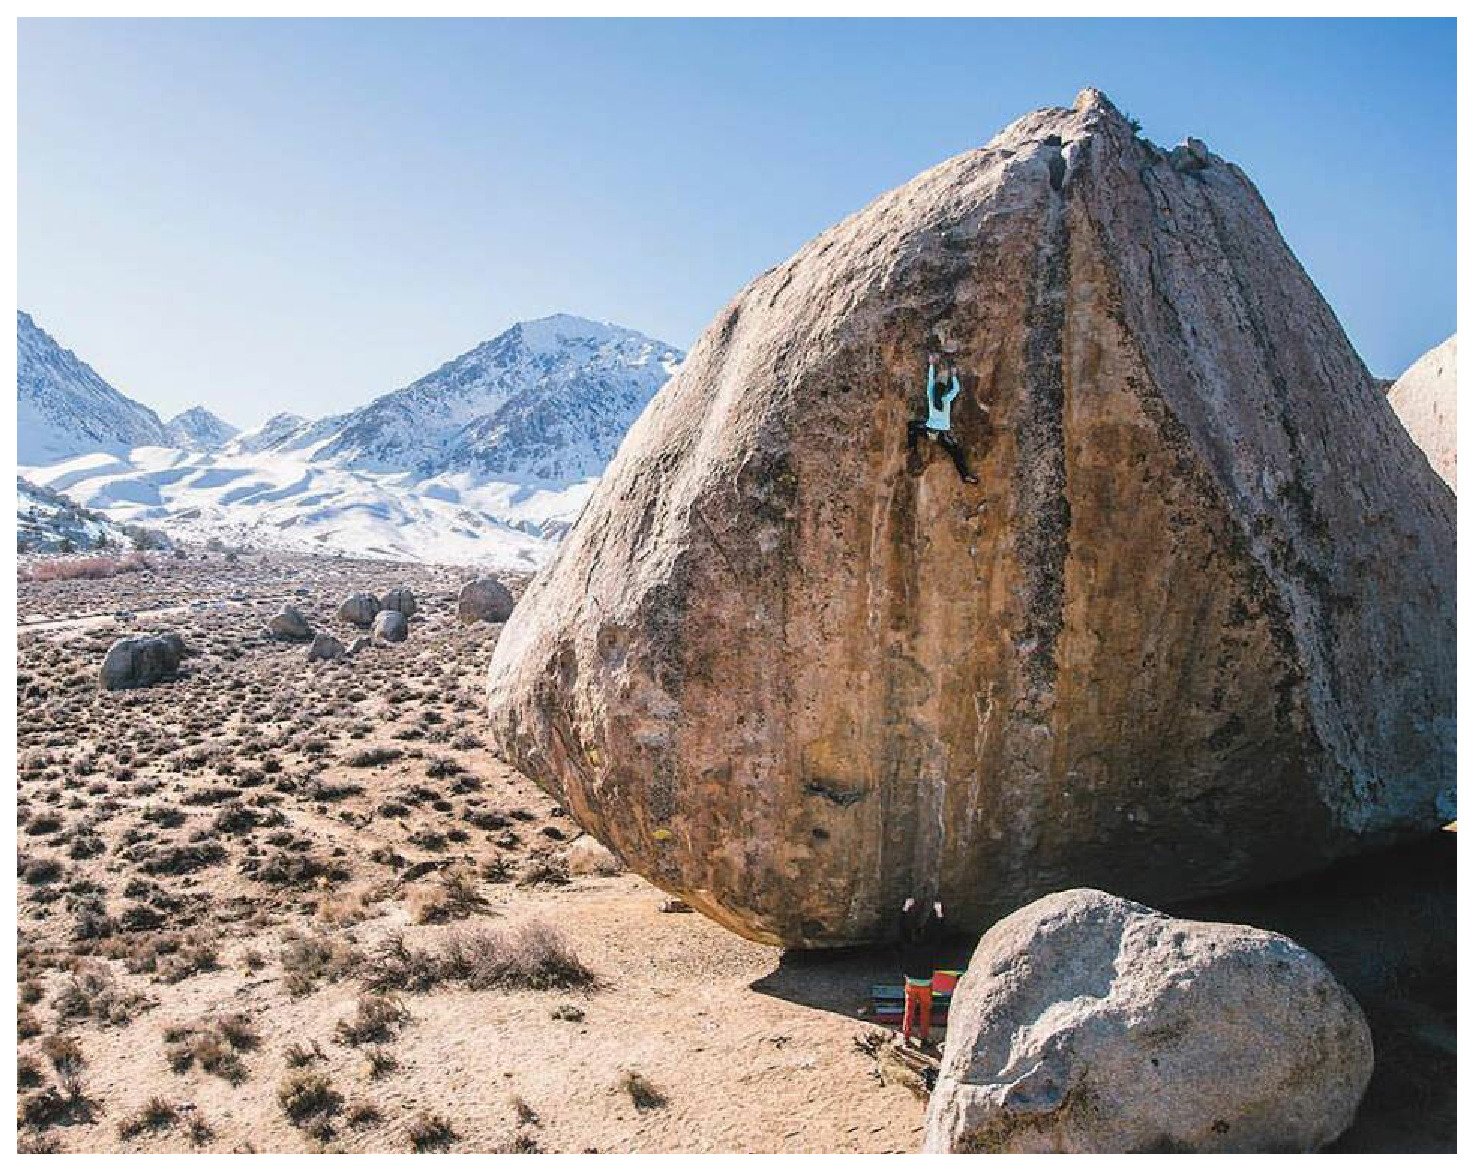
\includegraphics[width=0.7\linewidth]{images/nina-williams-abrosia.eps}
	\end{center}
	\caption{Nina Williams i słynny highball “Ambrosia” (fot. Nayton Rosales) \cite{nina}}
\end{figure}

\section{Historia}
\lettrine[lines=2]{S}{kupię} się na przedstawieniu światowej historii rozwoju omawianego w tej pracy sportu, jako że w dostępnych źródłach bardzo ciężko doszukać się informacji na temat polskiej historii boulderingu. Postaram się przytoczyć okoliczności powstania boulderingu, a następnie przejdę do przedstawienia jego obecnej sytuacji. Wspaniałym źródłem wiedzy o historii boulderingu okazały się materiały \cite{gill-history} napisane przez ojca współczesnego boulderingu - Johna Gill'a - o którym więcej napiszę w sekcji \ref{jg}. W tej pracy, nie jestem w stanie w tak dokładny i ciekawy sposób przekazać dostępnej tam wiedzy, dlatego zaciekawionego czytelnika zachęcam do zapoznania się z owymi materiałami - szczególnie interesującymi są liczne fotografie z przełomu XIX i XX wieku, ukazujące wspinaczy uprawiających czynności jak najbardziej przypominające bouldering (Rysunek \ref{benson}).

\begin{figure}[!htbp]
	\begin{center}
		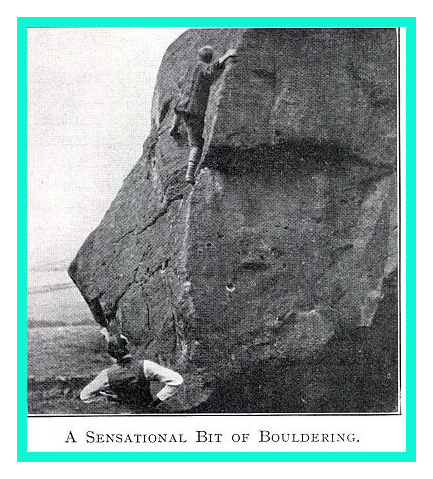
\includegraphics[width=0.5\linewidth]{images/old1.eps}
	\end{center}
	\caption{British Mountaineering, 1909 (fot. Claude E. Benson) \cite{gill-history}}
	\label{benson}
\end{figure}

\subsection{Początki}
Istnieją przypuszczenia, że początki nieudokumentowanego boulderingu sięgają drugiej połowy XIX wieku. Zaczynał wtedy rozkwitać alpinizm i gdy nie dopisywała pogoda, wspinacze mieli ćwiczyć na owych małych głazach jako przygotowanie do późniejszych ekspedycji. Mogliśmy takie praktyki najprawdopodobniej obserwować w m.im. \textit{Fontainebleau} we Francji, czy \textit{Lake District} w Wielkiej Brytanii. Niemniej jednak, takie podejście wspinaczy ukazywało bouldering jako środek do osiągnięcia "wyższych celi" i nie widziało w jego istocie sportu w pełnej okazałości. Ktoś mógłby rozsądnie i dociekliwie zatem zapytać, a z kiedy mamy pierwsze udokumentowane doniesienia o bardziej poważnym podejściu do rozważanej tutaj formy wspinaczki?

Na arenie międzynarodowej, to wspinacz Oscar Eckenstein, pochodzący z Wielkiej Brytanii, wydaje się być prekursorem boulderingu pokazującego oddanie tej dyscyplinie, zbliżone do tej które możemy obserwować w dzisiejszych czasach. Eckenstein żył na przełomie XIX i XX wieku i wspinał się m.in. w rejonie \textit{Lake District}. Aleister Crowley miał rzekomo mówić, że Eckenstein był w stanie pokonać problem na \textit{Y-Boulder} w \textit{Lake District} (rysunek \ref{collier}), którego inni wybitni wspinacze w ówczesnym momencie nie byli w stanie przejść. Zdaniem Johna Gill'a Eckenstein mógł być pierwszym prawdziwym mistrzem tego sportu - był wspinaczem, który nie tylko poszerzał standardy trudności, ale również w dość znaczący sposób przyczyniał się do ewolucji filozofii i praktykowania boulderingu. Niemniej jednak, większość brytyjskich wspinaczy dalej nie dostrzegała w tej formie wspinaczki oddzielnej dyscypliny.

\begin{figure}[!htbp]
	\begin{center}
		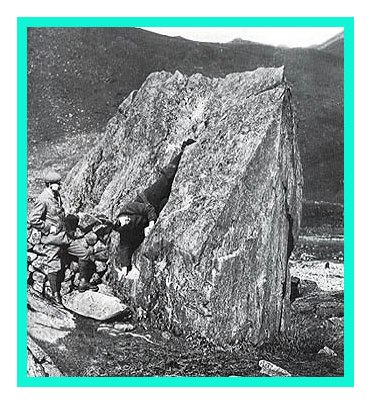
\includegraphics[width=0.5\linewidth]{images/y-boulder-collier.eps}
	\end{center}
	\caption{Dr Joseph Collier w trakcie próby przejścia \textit{Y-Boulder}, najprawdopodobniej pokonanej po raz pierwszy przez Oscara Eckensteina. Collier używa "wymaganej" tutaj techniki - próbuje pokonać fragment trasy do góry nogami (fot. George i Ashley Abraham) \cite{gill-history}}
	\label{collier}
\end{figure}

Dopiero w okresie międzywojennym Francuzi zaczęli eksplorować pomysł oddzielenia boulderingu od wspinaczki tradycyjnej, mowa tutaj o Pierre Allain, który wraz ze swoimi towarzyszami popularyzował wspinanie na gigantyczne głazy we francuskim \textit{Fontainebleau} (rysunek \ref{allain-1}). Po drugiej wojnie światowej mieli oni podobno dostrzegać wewnętrzną, nie motywowaną jedynie rozwijaniem umiejętności przydatnych do wypraw wysokogórskich, wartość wspinaczki w tym rejonie (rysunek \ref{allain-2}). Zdaniem Gill'a, Allain również zasługuje na miano mistrza tego jeszcze wtedy raczkującego sportu.

\begin{figure}[!htbp]
	\begin{center}
		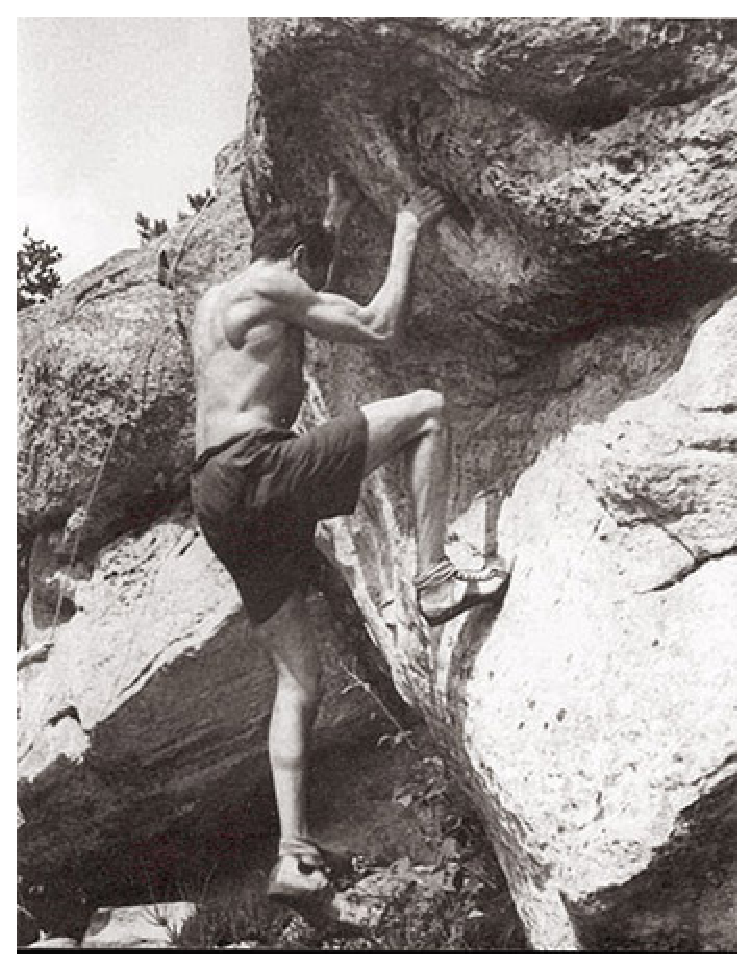
\includegraphics[width=0.5\linewidth]{images/allain-1.eps}
	\end{center}
	\caption{Pierre Allain w \textit{Fontainebleau} około roku 1938 (Editions Guerin-Chamoni) \cite{gill-history2}}
	\label{allain-1}
\end{figure}

\begin{figure}[!htbp]
	\begin{center}
		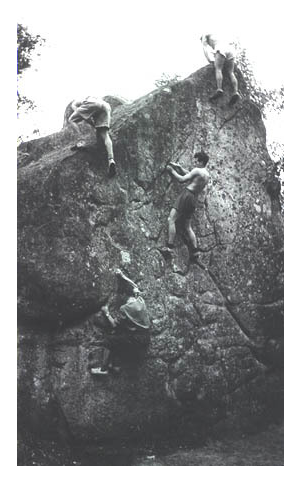
\includegraphics[width=0.35\linewidth]{images/allain-2.eps}
	\end{center}
	\caption{Pierre Allain i Guy Poulet kończący \textit{La Prestat Boulder} w \textit{Fontainebleau}. Po środku Rene Ferlet, a poniżej Jacques Poincenot. Około roku 1948 (Editions Guerin-Chamoni) \cite{gill-history2}}
	\label{allain-2}
\end{figure}

Podobny rozwój boulderingu można było obserwować w Wielkiej Brytanii. Zdaniem Gill'a na Wyspach Brytyjskich bouldering zyskał status zbliżony do obecnego dopiero w ostatniej ćwiartce XX wieku \cite{gill-history-1.2}. Parafrazując przemyślenia Geoffrey'a Winthropa Younga z książki \textit{Mountain Craft (1949)}: \textit{"Wprowadzenie do wspinaczki, którego zazwyczaj doświadczają nowicjusze, polega na ćwiczeniach na pojedynczych skałach, niskich klifach, czy też głazach, z lub bez użycia asekuracji na wędkę. Owy 'bouldering', czy też rozwiązywanie problemów, może służyć odkrywaniu talentu lub zachęcaniu do wspinaczki, ale jest mało użyteczne w trakcie rozpoczynania praktyki [...]"}. W książce \textit{Snowden Biography (1957)} możemy z kolei przeczytać, parafrazując: "\textit{Skały na niższych zboczach i wzgórzach nie były zupełnie brane pod uwagę jako dzień spędzony na prawdziwej wspinaczce. Ćwiczenie boulderingu, takie jak te które wykonywaliśmy w pobliżu naszej bazy, w dni wolne lub mokre, było ograniczonym ćwiczeniem, które niewiele przyczyniało się do poprawy techniki tamtych czasów. Dopiero gdy 'wspinaczkowa gorączka' rozprzestrzeniła się na obszary bez wzgórz, gdzie samotny kawałek żwiru lub piaskowca odgrywał rolę lokalnej góry, tak jak to miało miejsce w Peak District, bouldering, jak to nazywaliśmy, miał szansę rozwinąć się jako praktyka na dużą skalę i produkować swoich ekspertów [...]"} \cite{gill-history-1.2}.

\subsection{Nadejście współczesnego boulderingu}
Współczesny bouldering narodził się w latach 50-tych XX wieku, a za jego ojca można uznać Johna Gill'a (rysunek \ref{gill-1}). W odróżnieniu od wielu wspinaczy jego czasów, Gill szukał we wspinaczce bardziej pochodnej gimnastyki niż pochodnej wędrówki. Zainspirowany gimnastyką artystyczną, mianowicie jej kontrolowanymi ruchami dynamicznymi, zaczął owe ruchy ćwiczyć i wykorzystywać jako technikę pokonywania tras boulderowych. Ponadto, opracował pierwszy oddzielny system wyceny tras dla tej formy wspinaczki, i jak sam przyznaje, bardzo prawdopodobne, że był pierwszym w pełni specjalizującym się w boulderingu wspinaczem. Co więcej, starał się od początku promować bouldering jako oddzielny rodzaj wspinaczki, niezależny od konkretnej lokalizacji - w przeciwieństwie do poprzednich starań Pierre Allain'a, aby utożsamić tą formę aktywności z francuskim \textit{Fontainebleau}. Oprócz Gill'a w latach 60-tych w Stanach Zjednoczonych było jeszcze kilku wspinaczy, którzy widzieli w boulderingu samodzielną i autentyczną formę wspinaczki, o których warto tutaj wspomnieć - są nimi: Rich Goldstone, Pat Ament i Pete Cleveland. W latach 70-tych coraz więcej osób zaczęło skupiać swoją uwagę na wspinaniu się na "mniejsze głazy".

\begin{figure}[!htbp]
	\begin{center}
		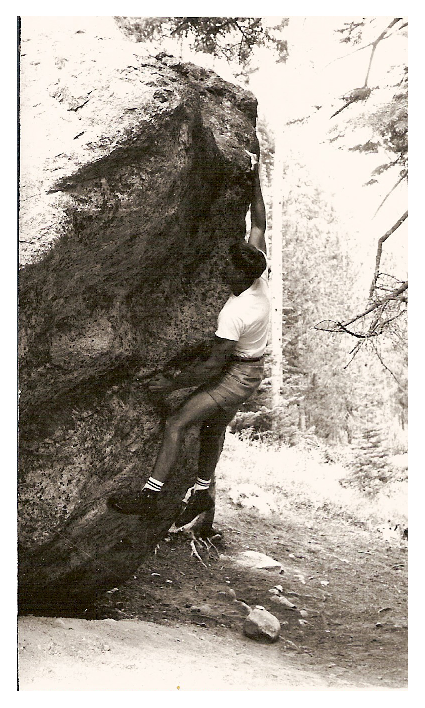
\includegraphics[width=0.5\linewidth]{images/gill-1.eps}
	\end{center}
	\caption{John Gill, \textit{Red Cross Rock Eliminate, V9}, 1963 \cite{gill-wiki}}
	\label{gill-1}
\end{figure}

W miarę rozwoju sportu, zaczęto dostrzegać ograniczenia skali trudności stworzonej przez Gill'a, była ona bowiem jedynie trójstopniowa. W latach 90-tych John Sherman zaproponował \textit{V-skalę} jako zamiennik skali Gill'a na użytek w \textit{Hueco Tanks} w Stanach Zjednoczonych. Jako, że okazała się ona bardzo użyteczna, została szeroko przyjęta w Ameryce. W Europie, z kolei, zdominowała skala francuska, pochodząca z \textit{Fontainebleau}. Co ciekawe, na początku współczesnego boulderingu używano okazjonalnego asekurowania na wędkę przy szukaniu rozwiązania problemów. Pod koniec XX wieku, spora większość wspinaczy zrezygnowała z tego sposobu na rzecz materacy i mat boulderingowych.

\subsection{Obecnie}
Największe zmiany jakich bouldering doświadczył od wejścia w okres swojej współczesności dotyczyły pojawienia się licznych krajowych i międzynarodowych zawodów, oraz związanej z tym standaryzacji i wzrostu ustanowionych limitów ludzkich możliwości. John Gill, używając skali z \textit{Hueco}, oszacował i porównał poziom najtrudniejszych tras na przestrzeni historii rozwoju boulderingu \cite{gill-history-1}. Gill szacuje, że około roku 1900 w Wielkiej Brytanii trudność tras wynosiła ok. V0-V1. Uważa z kolei, że Pierre Allain wraz ze swoimi kompanami dotarł w latach 30-tych XX wieku najprawdopodobniej do poziomu V3, a na przestrzeni kolejnych dwudziestu lat poziom w \textit{Fontainebleau} wzrósł do V4-V5. Poziom trudności swoich tras w późnych latach 50-tych, Gill plasuje pomiędzy V2 i V7, w porywach do V10. Na koniec, Gill stwierdza, że w latach 70-tych, Jim Holloway przekroczył najprawdopodobniej V12. Obecnie, najtrudniejszymi trasami są \textit{Burden of Dreams} i \textit{No Kpote Only} - obie z proponowanym poziomem trudności V17. Ale jak wyobrazić sobie poziom trudności tych tras? Jednym ze sposobów jest uświadomienie sobie ile pracy włożył w przygotowania Nalle Hukkataival - wspinacz który pierwszy, i do tej pory jedyny, przeszedł trasę \textit{Burden of Dreams}. Hukkataival miał podczas tamtego wyczynu na swoim koncie ok. 20 lat wspinaczkowego stażu, a same przygotowania do tej konkretnej trasy - opracowanie sposobu i zdobywanie odpowiedniej siły - zajęły mu ponad 3 lata \cite{hukkataival-yt}. Więcej o tym wspinaczu znajduje się w sekcji \ref{nh}. 

Szczególnie ważnym wydarzeniem dla boulderingu, i dla całego sportu jakim jest wspinaczka, było włączenie tej dyscypliny do Letnich Igrzysk Olimpijskich w roku 2020. Istnieje sporo kontrowersji co do wybranego formatu - każdy wspinacz musi jednocześnie konkurować w trzech, przez wielu uważanych za zupełnie inne, formach wspinaczki: wspinaczce sportowej z dolną asekuracją, boulderingu i wspinaczce na szybkość \cite{olympics}. 


\section{Znaczące postaci}
\lettrine[lines=2]{W}{tej} sekcji postaram się przedstawić sylwetki znaczących postaci ze względu na historię rozwoju boulderingu - John Gill, John Sherman i Fred Nicole, oraz sylwetki wspinaczy, którzy obecnie posiadają na swoim koncie najtrudniejsze trasy - wśród mężczyzn Nalle Hukkataival i wśród kobiet Ashima Shiraishi. 

\subsection{John Gill}
\label{jg}
\subsection{John Sherman}
\subsection{Fred Nicole}
\subsection{Ashima Shiraishi}
\subsection{Nalle Hukkataival}
\label{nh}
\nocite{*}
\printbibliography

\end{document}
